\chapter{Architectural Improvements in Generators and Discriminators}
As GANs have evolved, researchers have continually proposed architectural improvements to the generator and discriminator to enhance performance, particularly for high-resolution image generation~\cite{wang2018cgan, goodfellow2014generative}. One of the most influential approaches is Progressive Growing of GANs (ProGAN)~\cite{karras2017progressive}, which introduces a unique training strategy that significantly improves the quality of generated high-resolution images. In this chapter, we will explore the core ideas behind progressive training and how ProGAN achieves high-quality results, especially in generating large-scale images.

\section{Progressive Growing of GANs (ProGAN)}
Progressive Growing of GANs, introduced by Karras et al. in 2017~\cite{karras2017progressive}, is a method specifically designed to stabilize GAN training for high-resolution image generation. The idea is to gradually increase the complexity of the task by starting with a low-resolution image and progressively adding layers to both the generator and discriminator as training progresses. This gradual increase allows the network to learn the basic structure of the images at a low resolution before handling finer details, which significantly improves both training stability and the quality of the generated images~\cite{song2021gansim}.

\subsection{Core Idea of Progressive Training}
The core idea behind ProGAN is to train the GAN in phases, starting with small images (e.g., 4x4 pixels) and gradually increasing the resolution (e.g., 8x8, 16x16, 32x32, etc.) by adding layers to both the generator and discriminator.

\subsubsection{Progressive Layer Addition}
The training begins with a small resolution (e.g., 4x4 pixels). Once the network stabilizes at this resolution, new layers are added to both the generator and the discriminator, doubling the resolution (e.g., 8x8). This process continues until the desired resolution is reached (e.g., 1024x1024 for very high-resolution images). 

In each phase, the network learns to generate increasingly complex image features, starting with basic shapes and structures and progressing to finer details such as textures~\cite{karras2017progressive}. This progressive approach allows the model to focus on learning the essential structures of the image first, which leads to higher-quality results at larger resolutions~\cite{zhang2019progressive}.

\subsubsection{Fade-in Transition}
To avoid abrupt changes when new layers are added, ProGAN introduces a ``fade-in'' mechanism~\cite{zheng2022exploratory} during the transition between resolutions. Initially, when a new layer is added, its influence is weighted by a factor that gradually increases over time. This smooth transition helps maintain stability during training and prevents the network from being overwhelmed by the sudden increase in complexity~\cite{karras2017progressive}.

For example, if the network is transitioning from 8x8 to 16x16 resolution, the output from the new layers that handle 16x16 resolution is blended with the output from the previous layers (which handle 8x8 resolution) during the early stages of the transition. Over time, the contribution from the new layers increases until they fully take over.

\subsection{Improving the Quality of High-Resolution Image Generation}
The key benefit of ProGAN is its ability to generate high-quality, high-resolution images that maintain coherent global structure and fine details. This is achieved through a combination of architectural improvements and training strategies.

\subsubsection{Handling Large-Scale Data}
Generating large-scale images with traditional GAN architectures often leads to problems such as mode collapse, poor diversity, and instability~\cite{pathak2018efficient, kang2023scaling}. ProGAN overcomes these issues by training in stages, ensuring that the generator and discriminator learn to handle complexity progressively. By the time the model reaches high resolutions, it has already learned the core features of the data at lower resolutions, making it more stable and capable of producing diverse, realistic images~\cite{kang2023scaling}.

\subsubsection{Fine Details and Texture Learning}
As the resolution increases during training, ProGAN layers are able to focus on finer details, such as textures~\cite{ma1996texture} and edges, while preserving the overall structure of the image~\cite{dundar2023fine}. For example, in generating human faces, ProGAN can first learn the basic layout of facial features (eyes, nose, mouth) at low resolution and then gradually add details like skin texture, hair strands, and lighting effects as the resolution increases~\cite{dundar2023fine}.

\subsubsection{Training Stability}
Training GANs is often unstable, particularly when dealing with high-resolution images. The progressive training strategy of ProGAN helps alleviate this by simplifying the task in the early stages~\cite{dundar2023fine}. As the generator and discriminator are initially trained on small images, they can learn stable representations before tackling the more challenging task of generating high-resolution images. This reduces the likelihood of training collapse and leads to more consistent results~\cite{pathak2018efficient}.

\subsection{Step-by-Step Example of ProGAN using PyTorch}
To help you understand how ProGAN works in practice, let's walk through a simplified example using PyTorch. In this example, we will create a basic ProGAN-like architecture that starts with a small image resolution and progressively grows to handle larger resolutions.

\subsubsection{Step 1: Importing Necessary Libraries}
We first need to import the required libraries for our implementation:

\begin{lstlisting}[style=python]
import torch
import torch.nn as nn
import torch.optim as optim
import torch.nn.functional as F
from torch.autograd import Variable
import numpy as np
import matplotlib.pyplot as plt
\end{lstlisting}

\subsubsection{Step 2: Define the Generator and Discriminator}
In ProGAN, both the generator and discriminator architectures are designed to grow progressively as new layers are added during training. For simplicity, we will define basic versions of these models and then progressively add layers to them.

\begin{lstlisting}[style=python]
# Basic block used in both the generator and discriminator
class ConvBlock(nn.Module):
    def __init__(self, in_channels, out_channels, kernel_size=3, padding=1):
        super(ConvBlock, self).__init__()
        self.conv = nn.Conv2d(in_channels, out_channels, kernel_size, padding=padding)
        self.bn = nn.BatchNorm2d(out_channels)
        self.activation = nn.LeakyReLU(0.2)
    
    def forward(self, x):
        x = self.conv(x)
        x = self.bn(x)
        return self.activation(x)

# Generator model
class Generator(nn.Module):
    def __init__(self, latent_dim):
        super(Generator, self).__init__()
        self.initial_layer = nn.Sequential(
            nn.Linear(latent_dim, 128 * 4 * 4),
            nn.ReLU()
        )
        self.conv_blocks = nn.ModuleList([
            ConvBlock(128, 128),
            ConvBlock(128, 64),
            ConvBlock(64, 32)
        ])
        self.to_rgb = nn.Conv2d(32, 3, kernel_size=1, stride=1, padding=0)
    
    def forward(self, z):
        # Start with a 4x4 image
        x = self.initial_layer(z).view(-1, 128, 4, 4)
        for block in self.conv_blocks:
            x = F.interpolate(x, scale_factor=2)  # Upsample image progressively
            x = block(x)
        return torch.tanh(self.to_rgb(x))

# Discriminator model
class Discriminator(nn.Module):
    def __init__(self):
        super(Discriminator, self).__init__()
        self.conv_blocks = nn.ModuleList([
            ConvBlock(3, 32),
            ConvBlock(32, 64),
            ConvBlock(64, 128)
        ])
        self.fc = nn.Sequential(
            nn.Linear(128 * 4 * 4, 1),
            nn.Sigmoid()
        )
    
    def forward(self, x):
        for block in self.conv_blocks:
            x = block(x)
            x = F.avg_pool2d(x, kernel_size=2)  # Downsample image progressively
        x = x.view(x.size(0), -1)
        return self.fc(x)
\end{lstlisting}

Here, the generator starts by generating a small 4x4 image, which is progressively upsampled as it passes through the convolutional blocks. Similarly, the discriminator starts with a high-resolution image and progressively downsamples it before making a final classification.

\subsubsection{Step 3: Training Loop with Progressive Layer Addition}
Next, we define the training loop, where we progressively add layers to both the generator and discriminator as training progresses. We'll use a simplified version of ProGAN's fade-in mechanism to gradually introduce new layers~\cite{karras2017progressive}.

\begin{lstlisting}[style=python]
# Initialize models
latent_dim = 100
generator = Generator(latent_dim)
discriminator = Discriminator()

# Optimizers
optimizer_g = optim.Adam(generator.parameters(), lr=0.0002, betas=(0.5, 0.999))
optimizer_d = optim.Adam(discriminator.parameters(), lr=0.0002, betas=(0.5, 0.999))

# Training loop
epochs = 10
for epoch in range(epochs):
    for i, (real_imgs, _) in enumerate(dataloader):
        
        # Train Discriminator
        z = torch.randn(real_imgs.size(0), latent_dim)
        fake_imgs = generator(z)
        
        real_validity = discriminator(real_imgs)
        fake_validity = discriminator(fake_imgs.detach())
        
        d_loss_real = F.binary_cross_entropy(real_validity, torch.ones_like(real_validity))
        d_loss_fake = F.binary_cross_entropy(fake_validity, torch.zeros_like(fake_validity))
        d_loss = (d_loss_real + d_loss_fake) / 2

        optimizer_d.zero_grad()
        d_loss.backward()
        optimizer_d.step()

        # Train Generator
        fake_validity = discriminator(fake_imgs)
        g_loss = F.binary_cross_entropy(fake_validity, torch.ones_like(fake_validity))

        optimizer_g.zero_grad()
        g_loss.backward()
        optimizer_g.step()

    print(f"Epoch [{epoch}/{epochs}], D Loss: {d_loss.item()}, G Loss: {g_loss.item()}")
\end{lstlisting}

This basic training loop follows the usual GAN framework but with the additional concept of progressively increasing the resolution of generated images as new layers are introduced. In practice, this approach helps to stabilize training and allows the network to generate high-quality, high-resolution images over time.

\section{Summary}
In this chapter, we explored Progressive Growing of GANs (ProGAN), an important architectural innovation that significantly improves the stability and quality of GAN training, particularly for high-resolution image generation~\cite{karras2017progressive}. ProGAN's core idea is to train the GAN in phases, progressively increasing the resolution and complexity of the images. By starting with low-resolution images and gradually adding layers, ProGAN achieves more stable training and produces high-quality results. The use of fade-in transitions during layer addition further ensures smooth training progress. We also walked through an example implementation of ProGAN using PyTorch, providing a clear, step-by-step guide for beginners.










\section{BigGAN: Large-Scale Generative Adversarial Networks}
BigGAN~\cite{donahue2019large} is a powerful extension of the traditional GAN architecture, designed specifically to generate high-quality, large-scale images. Unlike traditional GANs that may struggle with larger, more complex datasets, BigGAN introduces several architectural and training improvements that allow it to generate realistic, high-resolution images on large-scale datasets such as ImageNet~\cite{deng2009imagenet}. This section will explain how BigGAN achieves this, and detail the techniques used to train it effectively`\cite{zhou2024comprehensive}.

\subsection{Generating High-Quality Large-Scale Images}
Generating high-quality, large-scale images is challenging because of the high complexity and variability present in real-world datasets. Traditional GAN architectures often produce blurry or low-quality images when scaled up to higher resolutions (e.g., \(256 \times 256\) or higher) or larger datasets (e.g., ImageNet). BigGAN addresses this problem by introducing several key innovations:

\textbf{1. Class-Conditional Batch Normalization:}  
BigGAN leverages class-conditional batch normalization (CCBN)~\cite{wang2020attentive} to condition both the Generator and Discriminator on class labels. In CCBN, the scale and shift parameters of the batch normalization layers are conditioned on the class label, allowing the Generator to produce images specific to a certain class, while still benefiting from the regularization properties of batch normalization~\cite{donahue2019large}.

\textbf{2. Larger Batch Sizes:}  
One of the fundamental challenges in GAN training is maintaining stability, especially as image resolution increases. BigGAN addresses this by utilizing larger batch sizes during training, which helps to reduce gradient noise and stabilize training. Larger batch sizes allow for more consistent updates to both the Generator and Discriminator, leading to higher-quality images~\cite{donahue2019large}.

\textbf{3. Orthogonal Regularization:}  
To prevent the Discriminator from becoming overly powerful and causing training instability, BigGAN applies orthogonal regularization to the weight matrices of the Generator. This prevents the weights from becoming too correlated, thus encouraging diversity in the generated images~\cite{wang2015deep}.

\textbf{4. Truncated Sampling:}  
BigGAN also introduces truncated sampling~\cite{brock2018large}, a method for controlling the diversity-quality tradeoff. Instead of sampling noise \(z\) from a normal distribution, BigGAN samples from a truncated normal distribution, which restricts the noise to a certain range. By limiting the noise input, the Generator is forced to focus on generating high-quality images that are more consistent with the target distribution~\cite{donahue2019large}. The truncation parameter can be adjusted to balance diversity and quality.

\textbf{Example: BigGAN Generator with Class-Conditional Batch Normalization in PyTorch}

\begin{lstlisting}[style=python]
import torch
import torch.nn as nn

# Class-Conditional BatchNorm2d
class ConditionalBatchNorm2d(nn.Module):
    def __init__(self, num_features, num_classes):
        super(ConditionalBatchNorm2d, self).__init__()
        self.bn = nn.BatchNorm2d(num_features, affine=False)
        self.embed = nn.Embedding(num_classes, num_features * 2)
        self.embed.weight.data[:, :num_features].normal_(1, 0.02)  # Scale
        self.embed.weight.data[:, num_features:].zero_()           # Shift

    def forward(self, x, y):
        out = self.bn(x)
        gamma, beta = self.embed(y).chunk(2, 1)
        gamma = gamma.view(-1, out.size(1), 1, 1)
        beta = beta.view(-1, out.size(1), 1, 1)
        return gamma * out + beta

# BigGAN Generator block
class BigGAN_GeneratorBlock(nn.Module):
    def __init__(self, in_channels, out_channels, num_classes):
        super(BigGAN_GeneratorBlock, self).__init__()
        self.conv1 = nn.ConvTranspose2d(in_channels, out_channels, 4, 2, 1)
        self.bn1 = ConditionalBatchNorm2d(out_channels, num_classes)
        self.relu = nn.ReLU(True)
        self.conv2 = nn.ConvTranspose2d(out_channels, out_channels, 3, 1, 1)
        self.bn2 = ConditionalBatchNorm2d(out_channels, num_classes)
    
    def forward(self, x, y):
        x = self.conv1(x)
        x = self.bn1(x, y)
        x = self.relu(x)
        x = self.conv2(x)
        x = self.bn2(x, y)
        return self.relu(x)

# Example usage
noise = torch.randn(16, 128, 1, 1)  # Noise vector
labels = torch.randint(0, 1000, (16,))  # Random class labels for 1000 classes
gen_block = BigGAN_GeneratorBlock(128, 256, 1000)
output = gen_block(noise, labels)
print(output.shape)  # Output should be torch.Size([16, 256, 4, 4])
\end{lstlisting}

In this example, the Generator block uses class-conditional batch normalization to condition the generation process on class labels. This is crucial for BigGAN's ability to generate diverse, high-quality images across many different categories.

\subsection{Training Techniques for Large-Scale Datasets}
Training a GAN on large-scale datasets like ImageNet presents several challenges, including the need for stable training, efficient resource utilization, and ensuring diversity in the generated images~\cite{donahue2019large}. BigGAN introduces several techniques to handle these challenges effectively:

\textbf{1. Gradient Accumulation for Large Batch Sizes:}  
BigGAN uses very large batch sizes (up to 2048 samples) during training, which can be resource-intensive. When the hardware cannot support such large batches in memory, gradient accumulation is used. Gradient accumulation involves accumulating gradients over multiple smaller batches and then updating the model parameters as if a larger batch was used. This allows the model to simulate training with a large batch size without the need for extensive hardware resources~\cite{brock2018large}.

\textbf{2. Self-Attention Mechanism:}  
To improve the generation of fine details and capture long-range dependencies in the images, BigGAN incorporates a self-attention mechanism~\cite{vaswani2017attention}. This helps the model focus on different parts of the image, allowing it to generate globally coherent images. The self-attention module is especially useful in generating high-resolution images where capturing global structure is critical.

\textbf{3. Spectral Normalization:}  
BigGAN also applies spectral normalization to both the Generator and the Discriminator. Spectral normalization helps to stabilize training by controlling the Lipschitz constant of the networks. This technique, already discussed in the context of SNGAN, is crucial for ensuring that the gradients do not explode or vanish, making it possible to train on large, complex datasets~\cite{donahue2019large}.

\textbf{4. Adaptive Learning Rates:}  
Since different layers of the Generator and Discriminator can have different magnitudes of gradient updates, BigGAN uses adaptive learning rates for different layers~\cite{ma2019adaptive}. This helps to balance the training dynamics and ensure that no single layer dominates the learning process.

\textbf{Example: Adding Self-Attention to BigGAN in PyTorch}

\begin{lstlisting}[style=python]
class SelfAttention(nn.Module):
    def __init__(self, in_channels):
        super(SelfAttention, self).__init__()
        self.query = nn.Conv2d(in_channels, in_channels // 8, 1)
        self.key = nn.Conv2d(in_channels, in_channels // 8, 1)
        self.value = nn.Conv2d(in_channels, in_channels, 1)
        self.gamma = nn.Parameter(torch.zeros(1))
    
    def forward(self, x):
        batch_size, C, width, height = x.size()
        query = self.query(x).view(batch_size, -1, width * height)  # B x C/8 x N
        key = self.key(x).view(batch_size, -1, width * height)      # B x C/8 x N
        value = self.value(x).view(batch_size, -1, width * height)  # B x C x N
        
        attention = torch.bmm(query.permute(0, 2, 1), key)          # B x N x N
        attention = torch.softmax(attention, dim=-1)
        
        out = torch.bmm(value, attention.permute(0, 2, 1))          # B x C x N
        out = out.view(batch_size, C, width, height)
        
        return self.gamma * out + x

# Example of using Self-Attention in BigGAN
class BigGAN_GeneratorWithAttention(nn.Module):
    def __init__(self, noise_dim, num_classes):
        super(BigGAN_GeneratorWithAttention, self).__init__()
        self.block1 = BigGAN_GeneratorBlock(noise_dim, 256, num_classes)
        self.attention1 = SelfAttention(256)
        self.block2 = BigGAN_GeneratorBlock(256, 128, num_classes)
    
    def forward(self, x, y):
        x = self.block1(x, y)
        x = self.attention1(x)  # Apply attention mechanism
        x = self.block2(x, y)
        return x

# Example usage
noise = torch.randn(16, 128, 1, 1)
labels = torch.randint(0, 1000, (16,))
gen = BigGAN_GeneratorWithAttention(128, 1000)
output = gen(noise, labels)
print(output.shape)  # Should output torch.Size([16, 128, 8, 8])
\end{lstlisting}

In this example, self-attention is integrated into the BigGAN architecture to capture global dependencies in the generated images, improving the quality of fine details and structure.

\subsubsection{Techniques for Efficient Training on Large Datasets}
To handle the complexity and size of large-scale datasets like ImageNet, BigGAN implements several advanced training techniques~\cite{adadi2021survey}:

\begin{itemize}
    \item \textbf{Multi-GPU Training:} To accommodate large models and batch sizes, BigGAN is often trained on multiple GPUs, distributing the workload and reducing training time.
    \item \textbf{Data Augmentation:} To improve generalization and prevent overfitting, BigGAN employs extensive data augmentation techniques such as random cropping, flipping, and color jittering.
    \item \textbf{Truncated Sampling:} Truncated sampling is used to improve the visual quality of generated images by controlling the range of noise inputs.
\end{itemize}

\textbf{Visualizing BigGAN's Training Process:}

\begin{center}
\begin{tikzpicture}
  [scale=1, every node/.style={scale=1}, 
  block/.style={rectangle, draw, fill=blue!20, text centered, minimum height=3em},
  arrow/.style={->, thick}]

  % Nodes
  \node[block] (noise) {Noise $z$};
  \node[block, right=of noise] (gen) {BigGAN Generator};
  \node[block, right=of gen] (gen_out) {Generated Images};
  \node[block, below=of gen_out] (disc) {BigGAN Discriminator};
  \node[block, below=of disc] (real_data) {Real Data};
  
  % Arrows
  \draw[arrow] (noise) -- (gen);
  \draw[arrow] (gen) -- (gen_out);
  \draw[arrow] (real_data) -- (disc);
  \draw[arrow] (gen_out) -- (disc);
\end{tikzpicture}
\end{center}

In this diagram, noise is passed through the BigGAN Generator to produce high-quality, large-scale images, which are then passed through the Discriminator for real vs fake classification. BigGAN applies techniques like self-attention and class-conditional batch normalization to ensure high-quality outputs.










\section{StyleGAN and StyleGAN2}
StyleGAN and its successor StyleGAN2~\cite{karras2020analyzing} represent a significant advancement in the field of GANs, particularly in terms of controllable image generation and high-quality results~\cite{khan2022transformers}. These models introduce innovative techniques such as style-based architecture and multi-resolution synthesis, which allow for fine-grained control over the features of generated images~\cite{bond2021deep}. In this section, we will explore the key concepts of StyleGAN and StyleGAN2, focusing on style control, multi-resolution generation, style mixing, feature interpolation, and their applications in image editing.

\begin{figure}[htbp]
    \centering
    \includegraphics[width=\textwidth]{figs/stylegan2.pdf}
    \caption{Example images and their projected and re-synthesized counterparts. For each configuration, top row shows the target images
    and bottom row shows the synthesis of the corresponding projected latent vector and noise inputs. With the baseline StyleGAN, projection
    often finds a reasonably close match for generated images, but especially the backgrounds differ from the originals. Image from Karras et al.\cite{karras2020analyzing} in 2020 StyleGAN2 paper.}
\end{figure}

\subsection{Style Control and Multi-Resolution Generation}

One of the main innovations in StyleGAN is its \textbf{style-based generator architecture}~\cite{karras2020analyzing}, which differs from traditional GANs. Instead of feeding the input noise directly into the generator, StyleGAN uses an intermediate latent space that allows for more structured control over the generated images. This architecture enables the separation of high-level and low-level features, leading to better control over the image generation process.

\subsubsection{Latent Space in StyleGAN}
In traditional GANs, a noise vector \( z \) sampled from a distribution (such as a normal distribution) is directly input to the generator~\cite{abdal2019image2stylegan}. However, in StyleGAN, the input noise \( z \) is first mapped to an intermediate latent space \( w \) using a learned function called a \textbf{mapping network}~\cite{karras2020analyzing}:
\[
w = M(z)
\]
Here, \( M \) is a multi-layer perceptron (MLP) that transforms the latent vector into a different space that is better suited for controlling image features. This allows for disentangling the features in a more intuitive way.

\subsubsection{AdaIN (Adaptive Instance Normalization)}
StyleGAN uses \textbf{Adaptive Instance Normalization} (AdaIN)~\cite{huang2017arbitrary} to control the style at different layers of the generator. AdaIN works by modulating the feature maps of the generator based on the style vector \( w \) for each resolution~\cite{kim2020transfer}. Specifically, AdaIN modifies the mean and variance of the feature maps at each layer using the style vector:
\[
\text{AdaIN}(x, y) = y_s \left( \frac{x - \mu(x)}{\sigma(x)} \right) + y_b
\]
Where:
\begin{itemize}
    \item \( x \) is the feature map.
    \item \( y_s \) and \( y_b \) are the style-specific scaling and bias values derived from \( w \).
    \item \( \mu(x) \) and \( \sigma(x) \) are the mean and standard deviation of the feature map.
\end{itemize}
By applying AdaIN at different layers, StyleGAN allows control over different levels of details in the generated image.

\subsubsection{Multi-Resolution Synthesis}
Another major innovation of StyleGAN is its ability to generate images at multiple resolutions, with fine control over different levels of detail. This is achieved by applying the style vector \( w \) at various stages of the generator, which corresponds to different image resolutions (e.g., low-level features like pose and shape at coarse resolutions, and high-level details like texture and color at finer resolutions)~\cite{jing2020dynamic}.

The generator starts by producing a low-resolution image, which is progressively upsampled to higher resolutions, with each stage adding more details. The style vector \( w \) controls the features generated at each resolution, providing fine-grained control over both global structure and local details.

\begin{lstlisting}[style=python]
# Example of AdaIN in PyTorch
import torch
import torch.nn as nn

class AdaIN(nn.Module):
    def __init__(self):
        super(AdaIN, self).__init__()

    def forward(self, content_features, style_features):
        content_mean, content_std = self._get_mean_std(content_features)
        style_mean, style_std = self._get_mean_std(style_features)

        normalized_content = (content_features - content_mean) / content_std
        return style_std * normalized_content + style_mean

    def _get_mean_std(self, features, eps=1e-5):
        size = features.size()
        mean = features.view(size[0], size[1], -1).mean(2).view(size[0], size[1], 1, 1)
        std = features.view(size[0], size[1], -1).std(2).view(size[0], size[1], 1, 1)
        return mean, std
\end{lstlisting}

In this code, AdaIN normalizes the content features (feature maps) using the statistics (mean and standard deviation) derived from the style features~\cite{karras2020analyzing}. This operation modulates the content features according to the desired style, as controlled by the latent vector \( w \).

\subsection{Style Mixing and Feature Interpolation}

\subsubsection{Style Mixing}

\textbf{Style mixing}~\cite{zhang2022styleswin} is another important concept introduced in StyleGAN, which allows for the combination of styles from multiple latent vectors to generate hybrid images~\cite{karras2020analyzing}. This technique helps the model learn more diverse representations and prevents overfitting to specific styles.

In style mixing, two different latent vectors \( w_1 \) and \( w_2 \) are used at different stages of the generator. For example, \( w_1 \) might be applied to the low-resolution layers, controlling global attributes like pose, while \( w_2 \) is applied to the high-resolution layers, controlling finer details like texture. This leads to images that inherit attributes from both latent vectors:
\[
\text{Generator}(w_1, w_2) = \text{AdaIN}(x, w_1) \quad \text{for low-res layers}, \quad \text{AdaIN}(x, w_2) \quad \text{for high-res layers}
\]

\begin{lstlisting}[style=python]
# Example of style mixing in PyTorch
def style_mixing(generator, w1, w2, mixing_point):
    """
    Apply w1 for layers up to mixing_point, and w2 for the rest.
    """
    for i, layer in enumerate(generator.layers):
        if i < mixing_point:
            style = w1
        else:
            style = w2
        x = layer.apply_style(x, style)
    return x
\end{lstlisting}

\subsubsection{Feature Interpolation}
Another powerful feature of StyleGAN is \textbf{feature interpolation}~\cite{upchurch2017deep}, which allows for smooth transitions between two different styles. This is done by interpolating between two latent vectors \( w_1 \) and \( w_2 \) and generating images that smoothly blend the characteristics of both.

The interpolation can be performed linearly between the two latent vectors:
\[
w_{interp} = \alpha w_1 + (1 - \alpha) w_2
\]
Where \( \alpha \in [0, 1] \) controls the blending ratio between the two styles.

\begin{lstlisting}[style=python]
# Example of feature interpolation in PyTorch
def interpolate_styles(generator, w1, w2, alpha):
    w_interp = alpha * w1 + (1 - alpha) * w2
    return generator(w_interp)
\end{lstlisting}

This allows for continuous transformations between different styles, providing rich possibilities for generating new images by blending features such as age, gender, or lighting conditions~\cite{karras2020analyzing}.

\subsection{Applications of StyleGAN in Image Editing}

StyleGAN has found significant applications in the field of \textbf{image editing}, where its ability to control specific attributes of an image makes it an incredibly powerful tool~\cite{bermano2022state}. Some of the key applications include face editing, attribute manipulation, and generating new artistic styles.

\subsubsection{Face Editing}
One of the most popular applications of StyleGAN is in generating and editing realistic human faces. By manipulating the latent vector \( w \), users can control attributes such as age, gender, facial expressions, hairstyle, and more~\cite{alaluf2022hyperstyle}.

For example, to change the age of a face, we can modify the latent vector in the direction corresponding to "age." This allows for intuitive editing of facial features.

\subsubsection{Attribute Manipulation}
In addition to face editing, StyleGAN can also be used to manipulate other attributes in generated images~\cite{patashnik2021styleclip}. For instance, StyleGAN can be used to adjust lighting conditions, change the background of a scene, or even mix different artistic styles (e.g., turning a realistic photo into a painting)~\cite{liu2023gan}.

\begin{lstlisting}[style=python]
# Example of attribute manipulation in PyTorch
def manipulate_attribute(generator, w, attribute_vector, intensity):
    """
    Manipulate a specific attribute by moving the latent vector w in the
    direction of the attribute_vector.
    """
    modified_w = w + intensity * attribute_vector
    return generator(modified_w)
\end{lstlisting}

In this example, the latent vector \( w \) is adjusted by adding the attribute vector (e.g., "smile" or "age") scaled by the desired intensity. This results in a modified image with the corresponding attribute altered.

\subsubsection{Artistic Style Transfer}
StyleGAN can also be employed in \textbf{artistic style transfer}~\cite{kotovenko2019content}, where features from one image (such as texture or color) are transferred onto another image. This can be done by using the style mixing technique, combining the structural features from one image with the artistic features from another.

\begin{center}
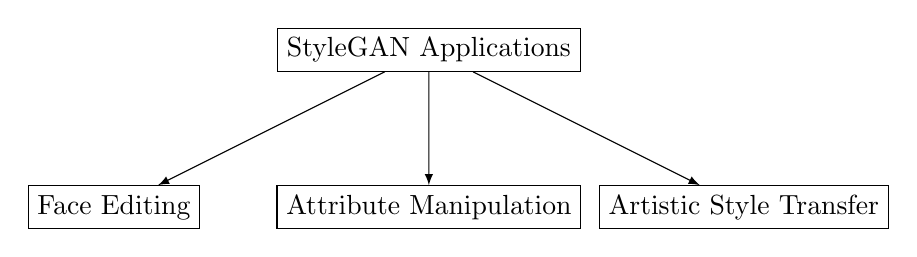
\begin{tikzpicture}[level distance=2cm, sibling distance=4cm, edge from parent/.style={draw,-latex}]
  \node[rectangle, draw] {StyleGAN Applications}
    child {node[rectangle, draw] {Face Editing}}
    child {node[rectangle, draw] {Attribute Manipulation}}
    child {node[rectangle, draw] {Artistic Style Transfer}};
\end{tikzpicture}
\end{center}

\subsubsection{Example: Editing Hair Style}
Suppose we want to change the hairstyle of a generated face. By manipulating the latent vector in the direction corresponding to "hair style," we can generate new images with varying hairstyles while preserving other facial features.

Here's how we can edit the hairstyle of a generated face using StyleGAN:

\begin{lstlisting}[style=python]
# Load pre-trained generator and latent vectors
generator = load_pretrained_stylegan()
latent_vector = sample_latent_vector()

# Hair style attribute direction
hair_style_vector = get_hair_style_direction()

# Modify latent vector to change hair style
modified_latent_vector = latent_vector + 0.5 * hair_style_vector
generated_image = generator(modified_latent_vector)
\end{lstlisting}

In this example, we add the hair style vector to the original latent vector, resulting in a generated face with a different hairstyle.

\section{Conclusion}

StyleGAN and StyleGAN2 represent a major leap forward in controllable image generation. Through techniques such as style-based generation, multi-resolution synthesis, style mixing, and feature interpolation, StyleGAN allows for fine-grained control over the characteristics of generated images~\cite{karras2020analyzing}. These capabilities have found broad applications in areas such as face editing, attribute manipulation, and artistic style transfer, making StyleGAN one of the most powerful and flexible GAN architectures available today.
